\documentclass[aip,cha,reprint,amsmath,amssymb]{revtex4-2}
\usepackage[utf8]{inputenc}
\usepackage[T2A]{fontenc}
\usepackage[english,russian]{babel}
\usepackage{bm}
\usepackage{graphicx}
\usepackage{hyperref}

\begin{document}

\title{Трёхпараметрический критерий встречного вращения и его проверка в двухчастичной RF-ловушке}
\author{Counterrotating Motion research project}
\date{24 ноября 2026 г.}

\begin{abstract}
Исследуется встречное среднее вращение двух заряженных частиц в математической модели двухчастотного поперечного поля 24-электродной ловушки. Для ведущих бегущих пространственных гармоник $k=+2$ и $k=-4$ независимо выводятся радиальный корень, критический радиус нулевого медленного RF-момента и тождество, исключающее радиус. В слабодиссипативном пределе получено условие $\max\{1,\alpha_2(1+\nu)\}<\Pi<1+\nu$, где $\Pi=\beta/(4A^2)$, $\alpha_1=1$, $0<\alpha_2<1$. Оно строго предсказывает противоположные знаки нулевого медленного момента при положительном допустимом радиальном корне; для переноса к стационарным скоростям дополнительно требуются существование моментного корня и положительное эффективное угловое сопротивление. Номинальный параметрический набор лежит внутри полосы. M0 предсказание согласуется с 33 из 36 ранее опубликованных одномерных M3 точек; расхождения находятся у почти нулевой скорости первой частицы. Уже опубликованная полная RF динамика подтверждает номинальную встречную ветвь и выбранные режимы по обе стороны крупного изменения амплитуды, но не точную границу перехода. M3 Fourier-collocation оценка даёт медианные числа Reynolds 0.332 и 1.605. Парное M3 решение с/без Schiller--Naumann нелинейности сохраняет знаки частот, но изменяет их модули на 25.8\% и 11.1\%. Полученные результаты описывают аналитический механизм и проверенные численные ветви, но не доказывают притягивающий тор полной RF системы или физическую реализуемость конечной ловушки.
\end{abstract}

\maketitle

\noindent\textbf{Lead paragraph.} Два заряженных объекта в одном вращающемся электрическом поле могут получать противоположный угловой момент, если разные отношения заряда к массе сначала помещают их на разные радиусы, а конкурирующие бегущие гармоники меняют относительный вес как $r^2$ и $r^6$. Мы выводим открытое трёхпараметрическое условие для знаков момента в ограниченной ведущей модели, проверяем его на опубликованных M3 ветвях и показываем, что нелинейное сопротивление существенно меняет частоты, хотя сохраняет их знаки на номинальном режиме.

\section{Введение}
Встречное вращение в общей ловушке можно объяснить без предположения, что кулоновская связь создаёт знаки движения. В рассматриваемой модели две независимые RF фазы возбуждают бегущие поперечные гармоники противоположной киральности. Различия $q/m$ меняют радиальную локализацию; при разных радиусах RF гармоники конкурируют с разным весом. Эта работа превращает указанную картину в проверяемый критерий и отмечает границы его действия.

Цель не состоит в сведении полной физической системы к трём независимым числам. При фиксированных геометрии, частицах, сопротивлении, Coulomb, MFS спектре и частоте первая ведущая система рассматривается в условном сечении $(A,B,\beta)$ и используется тройка $(\Pi,\nu,\alpha_2)$. Полная динамика содержит дополнительные независимые группы.

\section{Модель и ведущий радиальный баланс}
Пусть $\tau=\Omega_1t$, $\bm\xi_i=\bm r_i/R$, $\alpha_i=(q_i/m_i)/(q_1/m_1)$, $\alpha_1=1$, $\nu=\Omega_2/\Omega_1$. Вектор параметров refine12\_sobol17 и соответствующий восьмигармонический MFS спектр сохранены в исходном реестре V20B/V21A. Исторический полный RHS включает две RF фазы, Coulomb, тяжесть, DC квадруполь и Cunningham-corrected Stokes drag с Schiller--Naumann множителем. Поляризация выключена; поперечное поле соответствует бесконечно длинным электродам.

Для ведущих $+2,-4$ гармоник при нулевой средней орбитальной скорости и без Coulomb, радиального среднего drag и центробежного члена радиальный баланс равен
\begin{equation}
0=\alpha_i\beta r_i-\frac{4\alpha_i^2 A^2 K_{1i}}{D_{1i}}r_i
-\frac{48\alpha_i^2 B^2 K_{2i}}{D_{2i}}r_i^5,
\end{equation}
где $K_{1i}=1+\alpha_i\beta$, $K_{2i}=\nu^2+\alpha_i\beta$,
$D_{1i}=K_{1i}^2+\lambda_i^2$ и $D_{2i}=K_{2i}^2+(\lambda_i\nu)^2$.
Для ненормированных leading MFS коэффициентов нужны множители $|c_2|^2$ и $|c_{-4}|^2$ при $A^2$ и $B^2$ соответственно. Положительный конечный алгебраический корень требует $U_i>0$ и $V_i>0$, где
\begin{equation}
U_i=\alpha_i\beta-4\alpha_i^2 A^2|c_2|^2K_{1i}/D_{1i},\quad
V_i=48\alpha_i^2 B^2|c_{-4}|^2K_{2i}/D_{2i},\quad r_i^4=U_i/V_i.
\end{equation}
Кроме того, требуется $r_i+a_i/R<r_{\rm ap}/R$. Наклон скалярной радиальной силы в положительном корне при фиксированном нулевом спине равен $-4U_i<0$, но это не eigenvalue связанной радиально-угловой системы.

\section{Радиус-исключённое условие момента}
Для travelling mode степени $n=|k|$ полный RF момент и медленный орбитальный момент различаются: часть момента передаётся микродвижению, а его сопротивление также вносит torque. При нулевом среднем спине leading медленные моменты двух семейств имеют вид
\begin{equation}
\overline M_{\rm RF,total}=\sigma nP\frac{\lambda\nu_j}{D},\qquad
\overline M_{\rm slow}=\sigma(n-1)P\frac{\lambda\nu_j}{D},
\quad P=\alpha^2n^2|a_jc_k|^2r^{2n-2},\quad
D=(\nu_j^2+\alpha\beta)^2+(\lambda\nu_j)^2.
\end{equation}
Здесь $\sigma=\operatorname{sgn}(k)$, $\nu_j$ — частотное отношение RF семейства $j$, а $a_j$ — его ведущая амплитуда. Формулы относятся к линейному отклику при нулевой скорости среднего движения. Вторая формула получается вычитанием drag момента индуцированного микродвижения из полного RF момента; поэтому полный RF torque нельзя прямо принимать за torque медленной орбиты.
\begin{equation}
\mathcal T_i(0)=\frac{4\alpha_i^2 A^2|c_2|^2\lambda_i}{D_{1i}}r_i^2
-\frac{48\alpha_i^2 B^2|c_{-4}|^2\lambda_i\nu}{D_{2i}}r_i^6.
\end{equation}
Критический радиус — нуль этой суммы, а не нуль полного RF момента:
\begin{equation}
r_{\rm cr,i}^4=\frac{A^2|c_2|^2D_{2i}}
{12B^2|c_{-4}|^2\nu D_{1i}}.
\end{equation}
Деление $r_i^4/r_{\rm cr,i}^4$ с подстановкой радиального корня даёт
\begin{equation}
S_i=\frac{\nu}{K_{2i}}\left[
\frac{\beta D_{1i}}{4\alpha_i A^2|c_2|^2}-K_{1i}\right].
\label{eq:S}
\end{equation}
Ведущий $B^2|c_{-4}|^2$ сокращается, поскольку обе соответствующие силы пропорциональны $r^6$. Однако $B$ задаёт размер орбиты и допустимость корня, поэтому cancellation не означает физической независимости от $B$; предел $B\to0$ сингулярен.

В нормированном leading спектре $|c_2|=1$, в слабодиссипативном пределе $\lambda_i\ll1,\nu$, при $|\alpha_i\beta|\ll1$, $K_1\simeq D_1\simeq1$, $K_2\simeq\nu^2$, $D_2\simeq\nu^4$ имеем
\begin{equation}
S_i\simeq\frac{\Pi/\alpha_i-1}{\nu},\qquad \Pi=\frac{\beta}{4A^2}.
\end{equation}
Положительный корень для первой частицы требует $\Pi>1$; знак positive torque требует $S_1<1$, то есть $\Pi<1+\nu$. Для второй частицы $S_2>1$ означает negative torque, то есть $\Pi>\alpha_2(1+\nu)$. При $0<\alpha_2<1$ пересечение даёт открытый интервал
\begin{equation}
\boxed{\max\{1,\alpha_2(1+\nu)\}<\Pi<1+\nu.}
\label{eq:band}
\end{equation}
Условие (\ref{eq:band}) даёт знаки torque при нулевой средней скорости. Для stationary $\omega_i$ требуется существующий корень $\mathcal T_i(\omega_i)=0$ и $D_i^{\rm eff}=-\partial_{\omega_i}\mathcal T_i|_{\rm root}>0$; немонотонность или дополнительные корни требуют отдельной проверки.

\section{Номинальная точка и M3 сравнение}
Для refine12\_sobol17 получены $\Pi=3.1541817$, $\nu=3.2196774$, $\alpha_2=0.3781461$; M0 полоса составляет $1.5956545<\Pi<4.2196774$. С конечными $\lambda_i$ и DC поправкой (\ref{eq:S}) даёт $S_1=0.7521298$, $S_2=2.3886857$. Упрощённый M0 даёт $S_1=0.6690676$, $S_2=2.2800956$. Таким образом, номинальная пара попадает в $(+,-)$ torque область на обоих уровнях, но запас первой частицы до порога чувствителен к удержанным группам.

На номинальном M3 корне $r_1/R=0.5550375$, $r_2/R=0.7513383$, $f_1=+0.0547223$ Hz, $f_2=-0.0487398$ Hz. Полный M3 decomposition даёт RF family torques $+7.5171\cdot10^{-4},-3.6499\cdot10^{-4}$ для первой частицы и $+1.6793\cdot10^{-4},-2.6012\cdot10^{-4}$ для второй; нелинейный drag компенсирует каждую сумму на корне. Эти числа объясняют, почему результат не сводится к одному torque от Coulomb.

Из 36 сохранённых M3 continuation точек 33 согласуются с грубым знаковым прогнозом M0. Три отклонения приходятся на окрестность нулевого спина первой частицы, где M3 скорость мала. Ни solver failure, ни недостаток орбит у RF старта не интерпретированы как физическое отсутствие ветви. Полная RF кампания V21B подтверждает nominal $(+,-)$, $A=0.95A_0$ $(+,-)$ и $A=0.8A_0$ $(-,-)$; точки непосредственно у границы остаются неразрешёнными из-за недостатка оборотов.

\begin{figure}[t]
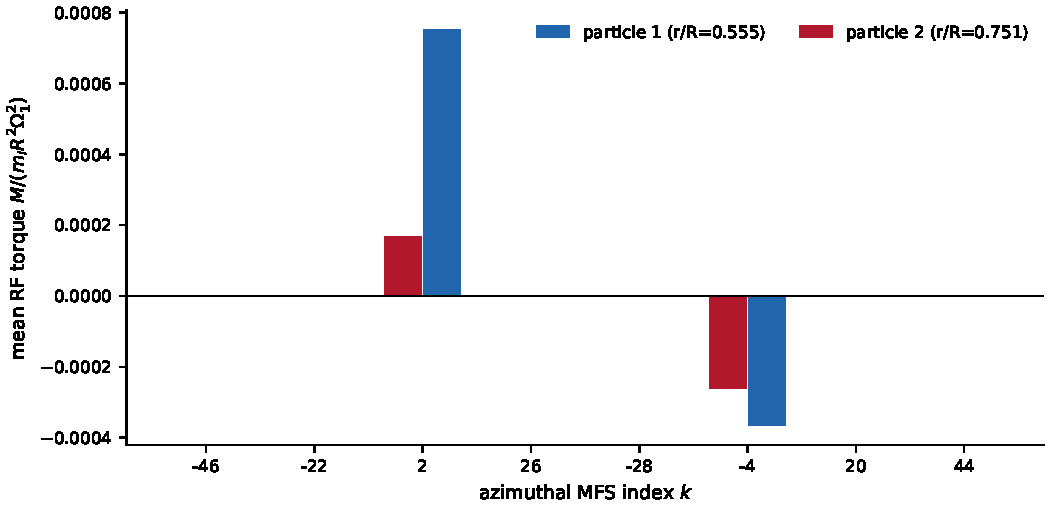
\includegraphics[width=\columnwidth]{figures/FIG01_m3_harmonic_torques.pdf}
\caption{M3 mean RF torque from each spatial harmonic at the nominal two-particle root.}
\label{fig:torques}
\end{figure}

\begin{figure}[t]
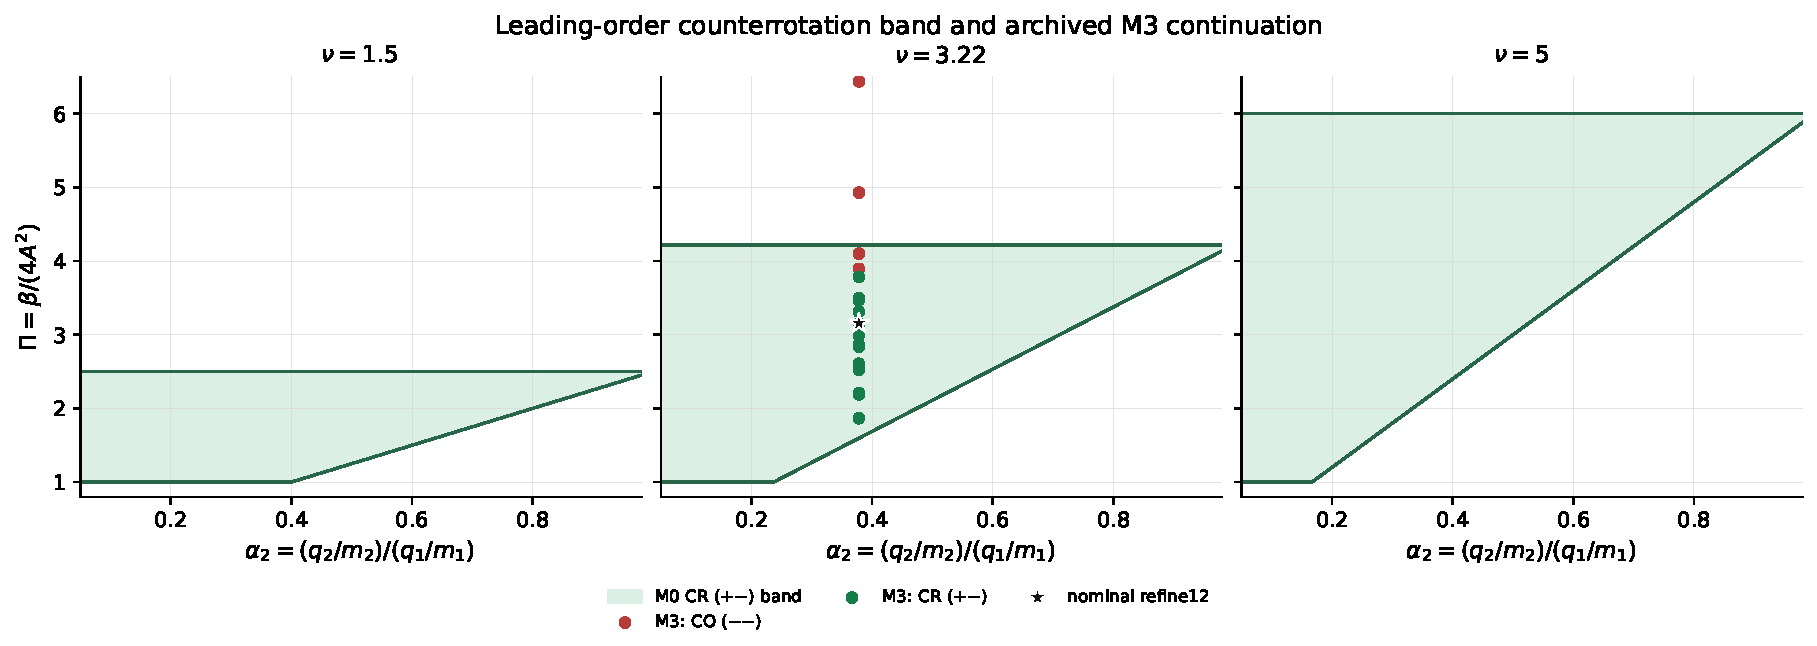
\includegraphics[width=\columnwidth]{figures/FIG03_three_parameter_M0_region.pdf}
\caption{Analytical M0 band on three fixed-$\nu$ sections. Sparse M3 branch points are shown only on the nominal-frequency section; they are not an independently sampled phase boundary.}
\label{fig:band}
\end{figure}

\section{Сопротивление Reynolds и численная проверка}
На фазовой сетке M3 192$\times$16$\times$16 с микродвижением медианные числа Reynolds равны 0.332 и 1.605; средние Schiller--Naumann множители — 1.0640 и 1.1944. Парные M3 solve на одинаковой сетке 96$\times$8$\times$8 с oversampling=2 дали для нелинейного drag частоты $+0.0547222,-0.0487402$ Hz и для линейного контроля $+0.0405961,-0.0433507$ Hz. Модули частот различаются на 25.8\% и 11.1\%, но знаки совпадают. Поэтому нелинейное сопротивление нельзя отбросить для количественного прогноза частоты, хотя номинальная направленность в этой паре сохраняется.

Новые тесты symbolic elimination, boundaries, leading MFS factors и независимой dimensional mapping: 9 тестов прошли. Полные RF решения не пересчитывались; использована опубликованная независимая V21B validation с 7 trajectories, 116000 RF1 periods и шаговым сравнением nominal 64/96 steps per period. Код, данные, CSV границы и рисунки находятся в архиве проекта.

\section{Область применимости и устойчивость}
M0/M1 не включают finite orbital speed, nonlinear harmonic coupling, высшие шесть MFS гармоник, Coulomb, radial drag и осевую связь. M2/M3 уменьшают эти ограничения, но точный boundary sweep полной M3 системы в трёхмерном пространстве $(\Pi,\nu,\alpha_2)$ не проводился. Локальный радиальный наклон не заменяет coupled stability. Долгоживущие полные RF решения и отрицательные собственные значения reduced M3 slow flow не доказывают притягивающий квазипериодический тор: текущий доказательный статус остаётся \texttt{LONG\_LIVED\_COUNTERROTATION}.

Кроме того, Chaos требует рукописи на английском языке и доступного неспециалисту lead paragraph; настоящий документ является русскоязычным проектным вариантом в Chaos/REVTeX формате, а не готовой английской submission version.\cite{chaosguide,revtexguide,v20barchive,v21archive}

\begin{acknowledgments}
Научные данные и код воспроизводят архивные версии V17C.20B, V17C.21A и V17C.21B. Авторский список, финансирование и declarations должны быть проверены ответственными авторами перед отправкой.
\end{acknowledgments}

\begin{thebibliography}{4}
\bibitem{chaosguide} AIP Publishing, ``CHA -- Editorial Policies,'' \url{https://pubs.aip.org/aip/cha/pages/policies}, accessed 24 November 2026.
\bibitem{revtexguide} AIP Publishing, ``Author Instructions,'' \url{https://pubs.aip.org/pages/author-instructions/}; AIP Substyles for REVTeX 4.2, \url{https://mirrors.ibiblio.org/CTAN/macros/latex2e/contrib/revtex/aip/aipguide4-2.pdf}.
\bibitem{v20barchive} Counterrotating Motion research archive, V17C.20B: particle dynamics, long trajectories and benchmark data, archived in repository branch `research/v17c20b-particle-attractor-search`, commit d1bf252649e174166becf464269318b5f97acd5d.
\bibitem{v21archive} Counterrotating Motion research archive, V17C.21A/B: M3 harmonic balance, continuation and selected full-RF validation, archived at source SHAs 94b8edfaac8a1f0b3eb518ea4c7594a80d47daf8 and 894c6896ce5927371708037ffa4a4021189d2b54.
\end{thebibliography}

\end{document}
